\documentclass[12pt]{article}
\usepackage[margin=1in]{geometry}
\usepackage{amsmath, amssymb, amsthm, tcolorbox, lastpage}
\usepackage{fancyhdr, accents}
\usepackage[natbibapa]{apacite}  

\usepackage{hyperref}
\usepackage{graphicx}
\usepackage{minted}


\pagestyle{fancy}
\setlength{\headheight}{40pt}

\newcommand{\ubar}[1]{\underaccent{\bar}{#1}}

\newcommand\tab[1][1cm]{\hspace*{#1}}

\title{CSC111H1-S Winter 2021 - Fundamentals of Computer Science 2 \\ Course Project Report}
\author{
  Ching Chang\\
  \and
  Letian Cheng\\
  \and
  Arkaprava Choudhury\\
  \and
  Hanrui Fan
}
\date{\today}

\begin{document}

\maketitle

\newpage

\lhead{Ching Chang, Letian Cheng \\ Arkaprava Choudhury, Hanrui Fan}
\rhead{CSC111H1-S Winter 2021 \\ Fundamentals of Computer Science 2 \\ Course Project Report}
\cfoot{\thepage\ of \pageref{LastPage}}

\begin{enumerate}
\item \section*{Part 1: Project Title and Group Members}
\textbf{Animmend - An interactive anime recommendation system.}

Ching Chang, Letian Cheng, Arkaprava Choudhury, Hanrui Fan

\newpage

\item \section*{Part 2: Problem Description and Research Question}
\begin{enumerate}
    \item \textbf{Overview of Background}
    
    \quad Anime is a genre of film and television animation that originated in Japan. Its wide range of storyline and unique art style has attracted over 20 millions audiences since 2018 \citep{Ani18}, and has been significantly scaling in multiple directions in the past 17 years \citep{Ell18}. With over 210 anime published last year in 2020 \citep{wiki21}, there are currently over 17,548 anime in the world \citep{MyA21} — way too many for anyone to pick!
    
    \item \textbf{Problem and Motivation}
    
    \quad This is a problem for both the audience and the producers of the anime who put in their blood and sweat into creating the work, only for it to be buried down in the monstrous pile of anime that are endlessly being published. Although there are anime-recommendation websites and applications out there that recommend users anime they might like based on their watch history, they tend to favour the trend and popular choices. This causes the established studios to self-perpetuate on the top of the pyramid scheme, while the rest that fails to make a good first impression end up at the bottom of the iceberg, forgotten. Much like every other film and television animation, anime is a form of fine arts medium where the authors, artists, and the production team splash their canvas with imagination and creativity. In a field with such freedom and originality, every anime has a meaningful story for someone in the world. Even the most terribly rated anime by the general could be a treasure to the right audience. However, it is difficult finding this so-called “right audience”. Anime with big names speak for themselves, so what the anime community lacks is a bridge between the unheard anime and the audience.
    
    \item \textbf{Our Goal}
    
    \quad To help mitigate this problem, we seek to create \textbf{an application that recommends unpopular anime based on the user’s input anime and relevant themes that they might be interested in.}
\end{enumerate}

\newpage

\item \section*{Part 3: Datasets}

\begin{itemize}
    \item Manami: An offline anime database \citep{manami}
    
    \textbf{Format:} This dataset's format is json. \href{https://gist.github.com/RealFakeAccount/cf34244d17039e78512428a1cf51d95f}{Data Example saved on GitHub}
    
    \textbf{Description:} 
    This source is used for retrieving each anime's title, thumbnail url, tags, and url to a webpage containing information about the anime. The rest of the data is ignored
    
    \item full.json: The parsed version of the Manami dataset, generated by our parse.py program
    
    \textbf{Format:} This dataset's format is json. 
    
    \textbf{Description:} This dataset is the output of parse.py. parse.py extracts the the title, url, thumbnail url, and tags of each anime from the original database and writes to a new json file. Note that anime with 0 tags will be removed
    
    \emph{A small sample of this dataset is called small.json}
    
    \item full\_graph.json: the serialize data of graph object
    
    \textbf{Format:} This dataset's format is json.
    
    \textbf{Description:} This dataset is the output of \emph{Graph.serialize} in Graph.py, and is used by the function \textit{load\_from\_serialized\_data} later. Since it takes roughly 17 seconds to calculate the similarity scores between all anime on 24 core cpu, we decided to calculate the similarity once, and save the results into a file that we can read from in the future.
    
    This file stores the attribute of the graph, \_anime: dict[str, Anime], which contains all attributes in the Anime class:
    
    \begin{minted}
        [
        frame=lines,
        framesep=2mm,
        baselinestretch=1.2,
        fontsize=\footnotesize,
        ]
        {python}
        
        title: str  # name of anime
        url: str  # url of anime on MAL
        thumbnail: str  # thumbnail
        detail: str  # introduction to the anime
        neighbours: list[str]
    \end{minted}

    \emph{We have a small sample of this dataset in small\_graph.json}
    
\end{itemize}
\newpage

\item \section*{Part 4: Computational Overview}

\begin{text}

\begin{itemize}
    \item parse.py
    \begin{itemize}
        \item parse\_json
        
            The \emph{parse\_json} function is used for processing the original Manami dataset. \textbf{New library, json, is used here} to read from and write to a json file. It opens the original Manami dataset, creates an empty dictionary, and add every part of the data we need (title, url, thumbnail, tags, and description) into the dictionary, while ignoring all the parts we do not need. After reading through the whole original json, we write the mutated dictionary into a new file.
            
        \item generate\_dataset
        
            The \emph{generate\_dataset} function is used for generate serialized dataset for the graph drawing. It initializes a graph and calculates the similarity score between every pair of anime, then serializes the data into a file.
            
        
        \item update\_graph
        
            The \emph{update\_graph} function is used for update graph based on previous user feedback.

    \end{itemize}

    
    \item Anime class in anime.py
    
    We used a graph structure to represent the collection of anime in our database. 
    
    Each vertex in the graph represents a single anime. We create a custom class “\texttt{Anime}” with public instance attributes including the anime's title (\texttt{str}), its review score on Manami (float), and a list of similar anime. We also include a private instance attribute, which is a dictionary mapping each relevant tag for the anime to a certain weighting. The dictionary is always normalized, i.e. the sum of the squares of the weightings is constant, which is implemented with the help of the helper function \texttt{normalize\_dict}. 
    
    We defined the ``similarity" of one anime with other anime as the sum of the products of the weightings corresponding to tags that both anime have in common. For instance, suppose that \texttt{a1} and \texttt{a2} have tags $t_1, \ldots, t_k$ in common with corresponding weights $w_{1,1}, \ldots, w_{1,k}$ in \texttt{a1} and $w_{2,1}, \ldots, w_{2,k}$ in \texttt{a2}. Then, we define:
    \begin{align*}
        similarity(a_1, a_2) &= \prod_{i=1}^k w_{1, i} \cdot w_{2, i}
    \end{align*}
    
    This approach is partly inspired by the vector space model used in search engines \citep{vspace}. The method \texttt{calculate\_similarity} in the anime class is a translation of this mathematical definition into Python code.
    
    As explained later in further detail, users can provide feedback on the recommendations, and the program automatically re-adjusts the weighting of each tag using vector normalization, and recomputes the similarity with other anime. This is done by the methods in the \texttt{Anime} class \texttt{adjust\_positive\_feedback} and \texttt{adjust\_negative\_feedback}. A positive feedback would increase the weightings of all relevant tags and a negative feedback decreases the weightings of all relevant tags.
    
    An anime's neighbours (i.e. the \texttt{neighbours} attribute) consists of the animes with the highest similarity with this anime.
    
    \item graph.py, Graph class and initialize graph

    There are several important functions in The \texttt{Graph} class.
    
    \begin{itemize}
        \item Graph.get\_anime\_description
        
            This function requires us to retrieve anime descriptions in real time, by making http requests. For that, \textbf{we use two new libraries: \textit{requests} and \textit{BeautifulSoup} here}. We first manually inspected the html structure of the websites that we are making the http requests to, and pre-defined the sections of the websites to parse from, for 4 different websites. As users click on the anime in our visualization, we will make http requests using the \textit{requests} library. With the returned data from the http requests, we then use \textit{BeautifulSoup} to parse and retrieve the description of the anime.
            
        \item Graph.serialize, load\_from\_serialized\_data, and Graph.\_add\_neighbour
        
            This function uses \textit{json} again in the same manner as we used it in \textit{parse.py}. We create an empty dictionary and iterate through each Anime in the graph, filling the dictionary with all the data contained in each anime, and write the dictionary into a json file. This is to save the loading time of running this program in the future, since calculating the similarity score between anime can take a very long time. By saving the graph data into a file (serializing), we can load directly from this data the next time we run the program, to avoid doing all the calculations again on initialization. Along with this method, we also implemented \textit{load\_from\_serialized\_data}, which uses \textit{json} to read from the serialized data, and construct the graph using it. Since the serialized data is obtained from the previous graph state, which is guaranteed to be a valid graph, we figured that it would be more efficient to modify \textit{Graph.add\_neighbour} from the implementation that we learned from class. From class, the method for inserting an edge between two vertices was to check that both vertices existed, then add each vertex to another one's set of neighbours. However, in our case, since we already know that the two vertices must exist (since the data is from the previous graph state), and we need to insert the neighbours in a specific order (descending similarity score), we modified the implementation such that \textit{Graph.add\_neighbour} is only one-directional. It only adds the anime associated to second parameter to the first parameter's list of neighbours, without adding the anime associated to the first parameter to the second parameter's list of neighbour. Calling this method on its own would seem error-prone, however, since we are using this method to load the serialized graph, it is error-free and more efficient.
            
        \item Graph.sort\_neighbours\_multiprocess
        
            This function uses \textit{multiprocessing} to speed up the calculation. This function needs to call Graph.\_sort\_neighbours, which has a time complexity of $\mathcal{O}(n \log n)$, $n$ times. We have around 30000 anime, and so, $n \approx 30000$. This should not be a big problem for languages like go and cpp. However, it takes more than 30 minutes for Python. To solve this problem, we rewrite this function using multiprocessing.Pool. We open a process pool with cpu.count() - 1 numbers of process (-1 is for stability). After using multiprocessing.Pool.map to auto assign each anime with process, We assign the result into the self.\_anime
            
        \item Graph.\_sort\_neighbours
        
            This function goes through the list of values in \texttt{Graph.\_anime} and uses sort with the callable \texttt{anime.calculate\_similarity} to sort out the most ``NEIGHBOUR\_LIMIT'' related animes for each anime.
            
        \item Graph.store\_feedback
        
            This function stores a tuple of user feedback into \texttt{Graph.\_feedback}. The tuple consists of three elements: the first element is the title of the current anime that the user searched for, the second element is the title of the anime that appeared in the recommendations, and the third element is the user response, which is either `upvote' or `downvote'.
        
        \item Graph.implement\_feedback
        
            This function implements the feedback that was stored in \texttt{Graph.\_feedback}. If \texttt{Graph.\_feedback} is not empty, we go through the feedback list in first-in first-out order. For each element in the list, we use the \texttt{Graph.adjust\_weighting} to change the weightings as needed.
        
        \item adjust\_weighting
        
            This function stores a tuple of user feedback into \texttt{Graph.\_feedback}. The tuple consists of three elements: the first element is the title of the current anime that the user searched for, the second element is the title of the anime that appeared in the recommendations, and the third element is the user response, which is either `upvote' or `downvote'.
        
        \item Graph.draw\_graph
        
            This function is perhaps the most important function in the file graph.py. It connects the processing of the content that we output to the user in the web page with the content that the user enters after interacting with it. In this function we use the title of the anime that the user wants to view, the depth of the anime associated with it and the maximum number of neighbours for each anime to generate the new graph. Here we introduce two new libraries: \textit{networkx} and \textit{plotly}. We determine the layout of the graph at the very beginning within the function, we don't need the graph to show the legend and axis information, but we determine the height of the graph on the page. We then create the set of visited animes, which allows us to traverse the neighbourhood of the user-selected anime with \textit{get\_related\_anime} without repeatedly visiting the anime, since the two animes are each other's neighbourhood. graph, we are going to add nodes to represent the different animes. The nodes store the string of the anime title so that other helper functions can better access the Graph's private variable \textit{\_anime} which has the type We also add edges to store the relationship of nodes of anime titles.
            
            We use a queue to implement this process. It is quite like BFS: the initialization pushes the core anime, which is the user's input, into the queue, together with the depth. In each while loop, we take the first node of the queue out, and iterate its loop to add nodes using \textit{self.add\_connection}. We then push the node into the end of the queue. The queue would become empty eventually, since the depth increase with the push operation.

            In order to allow users to visualize the hierarchical and neighborhood relationships of the graph and to take into account the aesthetics of the graph, we use \textit{spring\_layout} in \textit{networkx}, which is based on the Fruchterman-Reingold algorithm to arrange the nodes \citep{nxspr}. Currently we do not have anime without neighbors in our database, but of course we also consider the possibility of such a situation in subsequent updates, and set aside a separate drawing method to deal with the case of a node only without edge, the rest is the same as the design of the case diagram of multiple nodes. In the current interaction, we set the color of the central node to red and the other anime to blue, hovering over the points displays the title of the anime as well as the coordinates on the graph. On the edge represented by each gray line, we show the similarity of the anime at both ends of the edge that we obtained through our algorithm at the midpoint of the edge. This is all done through class \textit{Scatter} of \textit{plotly.graph\_objs} by passing the coordinates of each node calculated by \textit{spring\_layout} and midpoints of edges we calculated by \texttt{\_get\_all\_edges\_pos}.
    \end{itemize}

    \item visualization.py and interactive
    
        In visualization.py, this section uses a visual and interactive way to report our processing of the data and the computed graph, and we call the new library \textit{Dash} and its components \textit{dash\_core\_components} and \textit{ dash\_html\_components}, which are used to present all the components we have on the page. We introduced the Div component in \textit{dash\_html\_components} to wrap $<div>$ in html5, the Button component to wrap $<button>$ in html5 and the H5 component to wrap $<h5>$ in html5 and other components to wrap html5 elements \citep{Dashhtml}. We also use the Graph component of \textit{dash\_core\_components} to render any data visualization based on \textit{plotly}, the Slider component and the Dropdown component to create a slider for easy user input of values and a dropdown menu for inputting names of anime \citep{Dashdcc}.
        
        In visualization.py, we also have several functions to make changes to our web page by using \textit{callback} in \textit{Dash}. For example, \texttt{update\_graph} is used to update the graph generated on the right side of the interface based on user input. For two buttons on the top left side of the interface, \texttt{upvote\_downvote}is used to receive feedback from users on our recommended content and to update the \textit{json} file and \textit{full\_graph} after the program has been running for a while, using a background program to update the received feedback. \texttt{update\_name} is a function that helps to update name after user click on the graph to change new central node anime, co-working with \texttt{update\_graph}. \texttt{update\_description} is to help change description and thumbnail of anime based on what the user is hovering.
\end{itemize}

\end{text}

\newpage

\item \section*{Part 5: Instructions for obtaining datasets and running the program}

\begin{text}
WARNING: all our code are tested and verified under fresh ubuntu 20.04 with python3.9 and pip for python3.9 installed. Windows system might face some issues. If you face some strange issues about multiprocessing, please use Unix systems. Otherwise, you can choose not to run calc\_graph and use load\_from\_serialized\_data instead.

Please install all libraries under requirements.txt. Then,

Download the zip file using following credentials in UTsend:

Claim ID: CF88gEU9dbhgAMnJ

Claim Passcode: NotYkSiXVc2BZ7Pb

or download from following link: https://uoftctf.org/data.zip

After unzipping this file, you should have a data folder contains the following files:

\begin{itemize}
    \item full\_graph.json
    \item full.json
    \item original.json
    \item small\_graph.json
    \item small.json
\end{itemize}

Finally, for the main.py, you have several options: 

If you want to test the parse.py and generate data from scratch, uncomment the line that contains generate\_dataset

If you have made some feedback and want to regenerate graph, uncomment the line that contains update\_graph

Then dash will start a test server. It will automatically open a port. You should see "Dash is running on http://127.0.0.1:8050/" in your python console (the port you get might be different, just open the link in the browser).

Note: If you are running this program from more than one python console, you might get the following error:

OSError: [Errno 48] Address already in use

If that happens, just close the other consoles, and restart the program and make sure that you only run one process of this program at a time.

Once you open the link on the website, it should take a few seconds to load, and you should see the following:

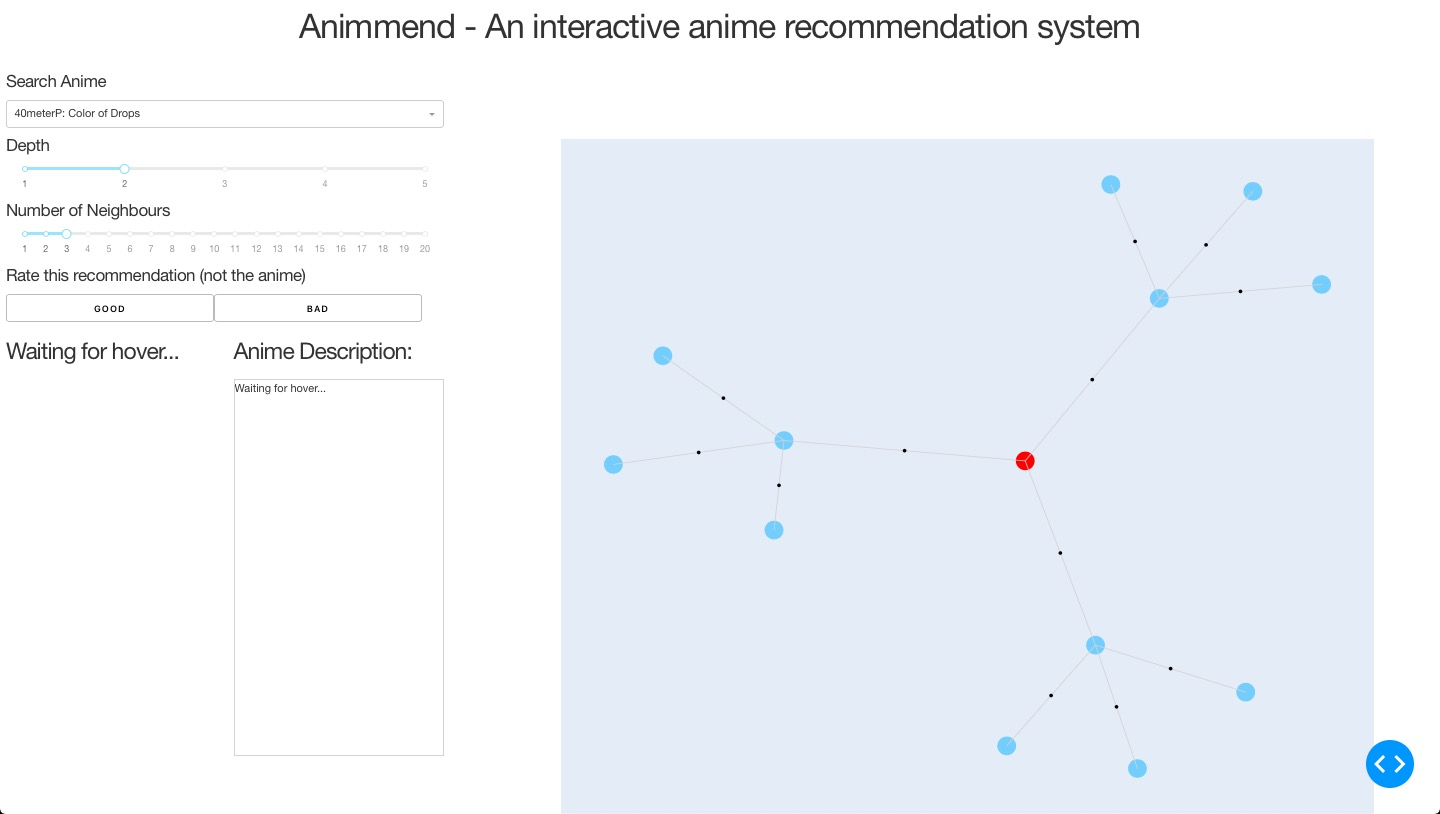
\includegraphics[scale=0.3]{initial.jpg}

On the left side, we have:

\begin{itemize}
    \item Search Anime: 

    You can select an anime from the dropdown menu, or type in an anime yourself. You cannot highlight or delete the text in the text box if you have selected from the dropdown menu, but as soon as you start typing, the text box is going to get cleared and update to what you typed

    \item Slider of depth: 

    You can change the depth of the graph to get more recommendations.

    \item Slider of neighbour:

    You can change the maximum number of edges for each vertex, which is the maximum number of similar anime that each anime extends into.

    \item Feedback:

    You can rate the quality of the recommendation of the anime that is currently being displayed (see anime description below) by clicking on one of the buttons (you rate the recommendation, not the anime itself!). The feedback might not cause an immediate change in the graph, but it will be taken into consideration for future recommendations

    \item Anime thumbnail/cover art
    
    \item Anime description:

    This is where the program displays the description of the hovered-anime by fetching it in real time. Note that the response time depends on your network connection, though it typically takes around 1s
\end{itemize}

The right side is a visualization of the graph. The red node in the centre represents the \textit{shell} of the graph (the anime that you searched for). The small black nodes store the similarity value of edge, which is measured from 0 to 1 (0 for no similarity, 1 for complete similarity). The blue nodes are the recommendations. You can click on the blue nodes to update the shell of graph.

If you would like to preview the blue nodes without updating the shell of the graph, simply hover over the blue nodes. Doing so will update the title, description, and the thumbnail on the left side, like the following example:

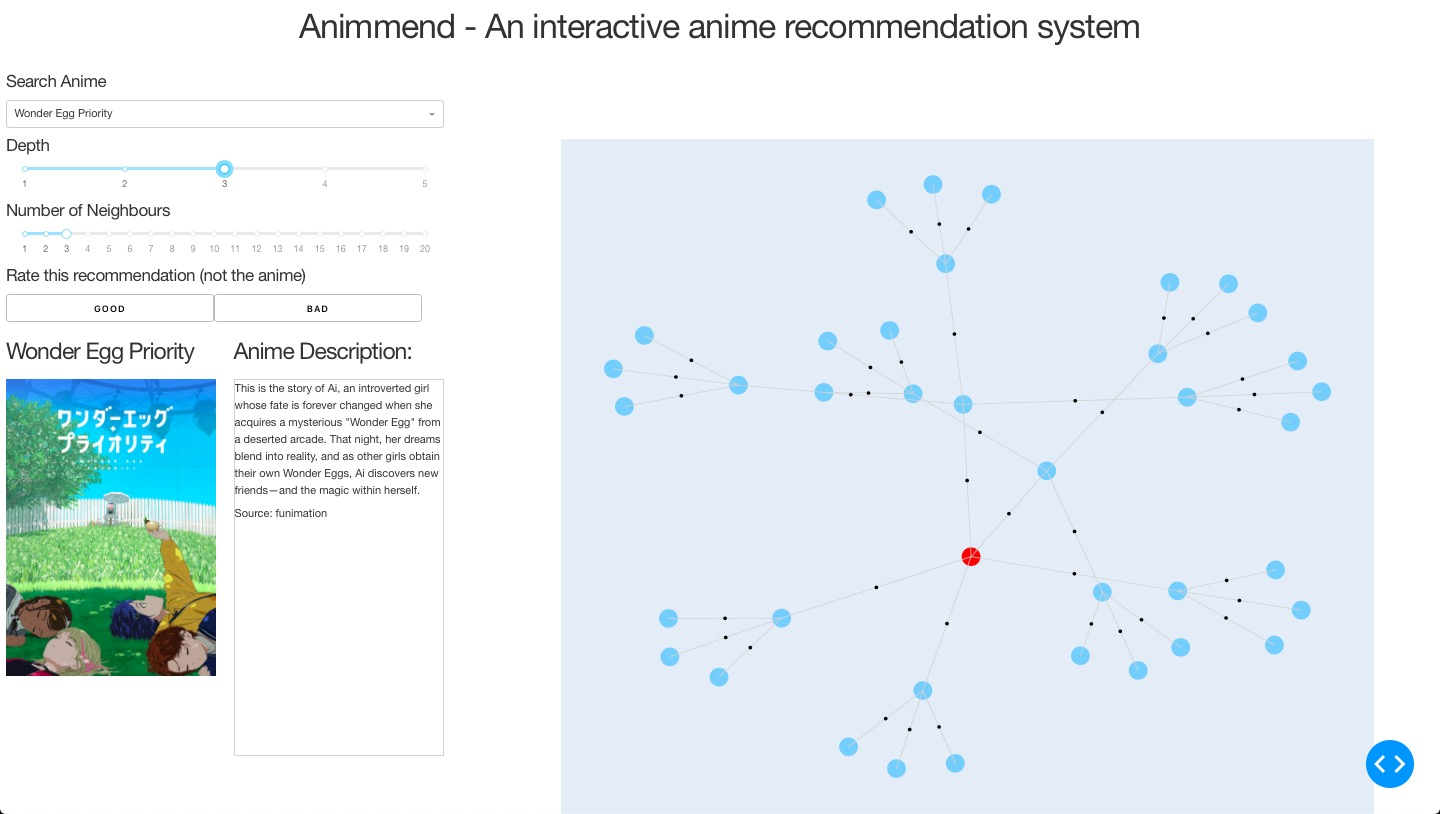
\includegraphics[scale=0.3]{egg.jpg}

\end{text}

\newpage

\item \section*{Part 6: Changes from Phase 1}

\begin{text}

\begin{enumerate}
    \item We no longer use lists to represent the tags for each anime, as we had described in the project proposal, and instead, we switched to representing the tags and their weightings as a dictionary. The rationale behind such a change was because we wanted to conserve storage space as we found out that there were more than 300 tags, and storing them in lists for each of the around 30000 anime was using up excessively large amounts of memory. A consequence of this change was the added benefit that we gained from constant-time look-up as compared to the $\Theta(n)$ worst-case running time of look-up using lists. Another advantage in this change was that it was less ambiguous than the previous idea, as we no longer referred to a predefined set order for the list, but rather, explicitly mentioned the tag and its weighting in the anime; in turn, this also makes it easier to introduce newer tags into the database without affecting the order of the other tags.
    
    The result of such a change implied that we could no longer use the built-in function \texttt{dot} in the \texttt{numpy} Python module, since that only works on array-like objects. We thus defined our own functions to calculate similarity of one anime with another, using an analogous definition as the dot product notation, as defined in Part 4. Consequently, we no longer use \texttt{numpy} in our project.
    
    \item We no longer explicitly store edges in a separate attribute \texttt{Graph.\_edges} as was done in the course. Instead, we store the neighbours of each node. We could assume that there are edges between the node and its neighbours. This simplify the coding complexity of \textit{draw\_graph}.
    
    \item We also revamped the way in which implemented the user feedback feature. A minor change was switching the terms `like' and `dislike' to `upvote' and `downvote' respectively, in favour of the existing nomenclature that is usually used in recommendation programs and social media. Besides this change in naming convention, we also made the feedback feature more user-friendly, by reducing the workload that is experienced by the user. Previously, we would have the user specify exactly which tags they agree/disagree with, for some anime in the recommendations. Currently, the user would only need to specify whether they agree/disagree with the recommended anime, and the program automatically recalculates the weightings of the tags that the recommended anime and the initial anime have in common. Although this increases the number of back-end calculations, we believe that it is a good change because it makes the recommendation system more intuitive for the users.
    
    \item We also made a greater use of serialization than we had planned in our project proposal. This was necessitated by the sheer size of the data that we were using. Similarly, we did not expect that we would need to use the \texttt{multiprocessing} library to speed up the process of initializing the graph with the data from the databases because we had not anticipated how long it would take for the program to work otherwise. This is because by default, python runs as a single process with a single thread of execution. Since modern computers often have a few even dozens of cores, this is a huge waste of efficiency. The \textit{sort\_neighbours} function happens to satisfy the requirement of multiprocessing and is easy to modify. Thus we use python's build in library - multiprocessing to rewrite it. The result is breathtaking: the time is more than 30 times less than the original function in 3900x.
\end{enumerate}

\end{text}

\newpage

\item \section*{Part 7: Discussion}

\begin{text}

\textbf{\emph{Discuss, analyse, and interpret your approach and the results of your program. Do the results of your computational exploration help answer research question?}}

The question of how ``similar" two anime are is always ambiguous and subjective. An art medium as free and creative as anime is filled with unquantifiable aspects such as the plot, art style, tone, theme, pacing, etc. There is no definitive way of judging the quality of similarity from an objective view, since what someone considers to be a criterion of similarity may be trivial in another person's criteria of similarity. Due to this limitation, the results of our program cannot be accurately evaluated in a global, bias-free manner. Rather, results are merely recommendations that, as our goal suggests, help popularize the less-known anime. With this as the primary goal, we consider a recommendation to be successful if it
\begin{enumerate}
    \item is an anime that we have never heard of, AND
    \item sparks our interest
\end{enumerate}
Using this definition, our group concluded that our program is moderately successful at achieving the project goal, given that every recommendation that we received did surprisingly satisfy the two criteria (Note: this evaluation is subjected to the small-sample bias). However, our results are displayed in a visually overwhelming way. Users are unlikely to increase the depths and edges, and properly consider every single recommendation that we provide. This limits the effectiveness of popularizing anime such that an estimate of only $\sim5$ anime are actually being considered by the user per search (Note: this is also subjected to the small-sample bias). It is ineffective at popularizing unpopular anime over a night, but we do believe that it has the potential of slowly bringing unpopular anime to the light over a longer period.

One challenge that we faced early in the project was the exact definition of similarity to use. We noticed that in almost all anime databases, anime were characterized by their `tags', i.e. their genres, which meant that this was an obvious choice for how to `describe' an anime. We thus decided to use this as a basis for determining the similarity of an anime. In more linear-algebra-esque terms, this quite literally forms a basis for the `tag' vectors, as we had described in the project proposal, with each anime being represented as some vector in the vector space defined by this basis. The advantage of such a definition relied on the assumption that people usually tend to enjoy items from the same genres, and so, such items would often be good recommendations. However, the limitation of such an approach would be that it fails to take into account factors such as animation style, soundtrack composer, animation studio, voice actors, etc, which several users might otherwise take into account while deciding their anime watch-lists.

Now, after going through our datasets, we found out that there were far more tags than we had previously imagined, and storing the `tag vector' for each anime in the form of a list would be quite infeasible in terms of the memory it would use. Ultimately, we settled on using a dictionary to represent the tags, as explained in Part 6. Now, in our earlier versions, we had not normalized all the weightings for the anime, which led to problems when comparing the similarity across different anime, so clearly, we needed to settle on some normalization scale. Ultimately, we decided on using the standard real Euclidean inner product defined on all finite-dimensional real Euclidean spaces \citep{Euclinn}, as such a definition agreed perfectly with the vector space analogy explained earlier.

A large advantage of our implementation of the anime recommendation system is that we store zero details about the user, which could potentially reveal their identity. This may seem like a trivial fact, especially given the problem domain, but identity theft is nonetheless a very prominent and dangerous risk of online interactions.

\bigskip

\textbf{\textit{What limitations did you encounter, with the datasets you found, the algorithms/libraries you used, or other obstacles?}}

The largest problem that we faced was retrieving the anime description. We initially planned on finding a database or an application programming interface (API) for the anime description, but quickly found out that such a database or API does not exist, or was too difficult to find. Our second approach was to scrape websites that contain anime descriptions, and put them together to generate our own data. We implemented this feature using the requests and BeautifulSoup libraries in a similar way as what is shown in our, except that the function was designed to fetch every anime in the database and serialize them before for all future graphs. However, this approach failed since some websites that we scrape from disallowed bots and blocked us from making more requests from them. In addition, this approach was also very slow. To mitigate all these issues, our final solution was to only fetch the anime description when the user hovers over the anime. This helped us reduce the number of requests we make to the site, while also giving us the most up-to-date description, at the cost of a $\sim1$s wait time.

\bigskip

\textbf{\textit{What are some next steps for further exploration?}}

Moving forward, we plan to take the following steps to improve upon this project:

\begin{enumerate}
    \item Currently, our implementation of similarity is not ``symmetric", in the following sense. Let $a_1, a_2$ be two anime in our dataset. Suppose that $a_2$ is included in the list of neighbours of $a_1$. However, it doesn't follow that $a_2$ must be included in the list of neighbours of $a_1$, since there may be other anime, say $b_1, \ldots, b_k$ where $k \geq$ NEIGHBOUR\_LIMIT. In effect, the current implementation of \texttt{Graph} is actually a directed graph, and not an undirected graph. To convert this into an undirected graph, we can simply introduce a stricter subclass of \texttt{Graph}, called \texttt{StrictGraph}, which would involve re-defining the list of neighbours such that it is symmetric. In other words, \texttt{StrictGraph} should include $a_2$ in the list of neighbours of $a_1$ if and only if $a_1$ is included in the list of neighbours of $a_2$. A naive translation of this implementation would involve over-writing \texttt{draw\_graph} such that it adds an undirected edge between \texttt{a1} and \texttt{a2} if \texttt{a1 in a2.neighbours} and \texttt{a2 in a1.neighbours}.
    
    The reason why we stress on the definition of similarity and invoking similarity is because we could then include ...
    \item We also plan on improving the prediction functions such that, among the list of recommendations, we are able to point out certain anime that the user is likely to pick next. As is the case with all prediction algorithms, since human nature is complex and seemingly random, thoroughly testing whether such a feature works would necessitate randomized testing with certain sample groups.
    
    The advantage of including such a feature lies in the fact that our program could then learn more about the user's interests and, over time, adapt to recommending anime that would be more likely to pique the user's interests. In doing so, we would be creating a program that can be personalized to each user.
    \item Currently, our mutating of the graph is rather inefficient as we recalculate the entire graph while doing so. We could potentially speed up this process in the average-case scenario by utilizing approximation algorithms to estimate which vertices and nodes would remain unchanged, which would reduce the time and space complexity of our code.
    
    This could potentially involve finding clusters in the anime graph along with strongly connected components, thus effectively reducing the size of the graph used in certain cases, leading to a speed-up in the program.
\end{enumerate}

Furthermore, we should also implement an automated system that periodically adds new anime into the database. We can do so by keeping the program running, and making a monthly http request to the list of anime on myanimelist.net, sorted by ``new". Every time we do so, we store the newest 50 anime, and check if any of them is not in the list from the previous month.
\end{text}


\maketitle

\newpage

\bibliography{references}
\bibliographystyle{apacite}

\end{enumerate}

\end{document}